\documentclass[10pt]{beamer}

%% Based on the original theme by Matthias Vogelgesang

\usetheme[progressbar=frametitle]{metropolis}
\usepackage{appendixnumberbeamer}

\usepackage{booktabs}
\usepackage[scale=2]{ccicons}

\usepackage{pgfplots}
\usepgfplotslibrary{dateplot}

\usepackage{xspace}
\newcommand{\themename}{\textbf{\textsc{metropolis}}\xspace}

%%%%%%%%%%%%%%%%%%%%%%%%%%%%
%% UNCC Theme Adjustments %%
%%%%%%%%%%%%%%%%%%%%%%%%%%%%
\definecolor{CanvasBG}{HTML}{FAFAFA}

% From the official style guide
\definecolor{UnccGreen}{HTML}{00703C}
\definecolor{UnccGold}{HTML}{B3A369}
\definecolor{UnccLightGreen}{HTML}{C3D7A4}
\definecolor{UnccYellow}{HTML}{F0CB00}
\definecolor{UnccOrange}{HTML}{F3901D}
\definecolor{UnccLightYellow}{HTML}{FFF6DC}
\definecolor{UnccBlue}{HTML}{00728F}
\definecolor{UnccPink}{HTML}{DE3A6E}
\definecolor{White}{HTML}{FFFFFF}
\definecolor{LightGray}{HTML}{DDDDDD}

% Supporting Color Palette
\definecolor{WarmGray}{HTML}{696158}
\definecolor{StoneGray}{HTML}{717C7D}
\definecolor{DarkGreen}{HTML}{2C5234}
\definecolor{LightGreen}{HTML}{509E2F}
\definecolor{BrightGold}{HTML}{F0CB00}

% Screamers
\definecolor{Royal}{HTML}{72246C}
\definecolor{Ocean}{HTML}{006BA6}
\definecolor{Flash}{HTML}{B52555}
\definecolor{Citrus}{HTML}{FFB81C}
\definecolor{Spring}{HTML}{CEDC00}

% Serenity
\definecolor{Garden}{HTML}{B7CE95}
\definecolor{Sand}{HTML}{F0E991}
\definecolor{Bloom}{HTML}{F1E6B2}
\definecolor{Clay}{HTML}{B7B09C}
\definecolor{Cloud}{HTML}{BAC5B9}

% Set colors here
\setbeamercolor{frametitle}{bg=UnccGreen}
\setbeamercolor{progress bar}{bg=BrightGold, fg=UnccGreen}
\setbeamercolor{alerted text}{fg=Flash}

\setbeamercolor{block title}{bg=LightGreen, fg=White}
\setbeamercolor{block title example}{bg=Ocean, fg=White}
\setbeamercolor{block title alerted}{bg=Citrus, fg=White}
\setbeamercolor{block body}{bg=CanvasBG}

\metroset{titleformat=smallcaps, progressbar=foot, sectionpage=none}

\makeatletter
\setlength{\metropolis@progressinheadfoot@linewidth}{2pt}
\setlength{\metropolis@titleseparator@linewidth}{2pt}
\setlength{\metropolis@progressonsectionpage@linewidth}{2pt}
%%%%%%%%%%%%%%%%%%%%%%%%%%%%
%% UNCC Theme Adjustments %%
%%%%%%%%%%%%%%%%%%%%%%%%%%%%


\title{Antrittsvortrag}
\subtitle{Handgestenerkennung mit Entscheidungsbäumen}
% \date{\today}
\date{}
\author{Tom Dymel}
\institute{Technische Universität Hamburg}
% \titlegraphic{\hfill\includegraphics[height=1.5cm]{logo.pdf}}

\begin{document}

\maketitle

\begin{frame}{Table of contents}
  \setbeamertemplate{section in toc}[sections numbered]
  \tableofcontents[hideallsubsections]
\end{frame}

\section{Motivation}
\begin{frame}{Motivation}
\begin{itemize}
    \item Zuverlässige Gestenerkennung
    \item Preiswertes Modul
    \item Echtzeit-Evaluierung 
\end{itemize}
\end{frame}

\section{Optische Handgestenerkennung}
%Kurz!
\begin{frame}{Optische Handgestenerkennung}
\begin{figure}
    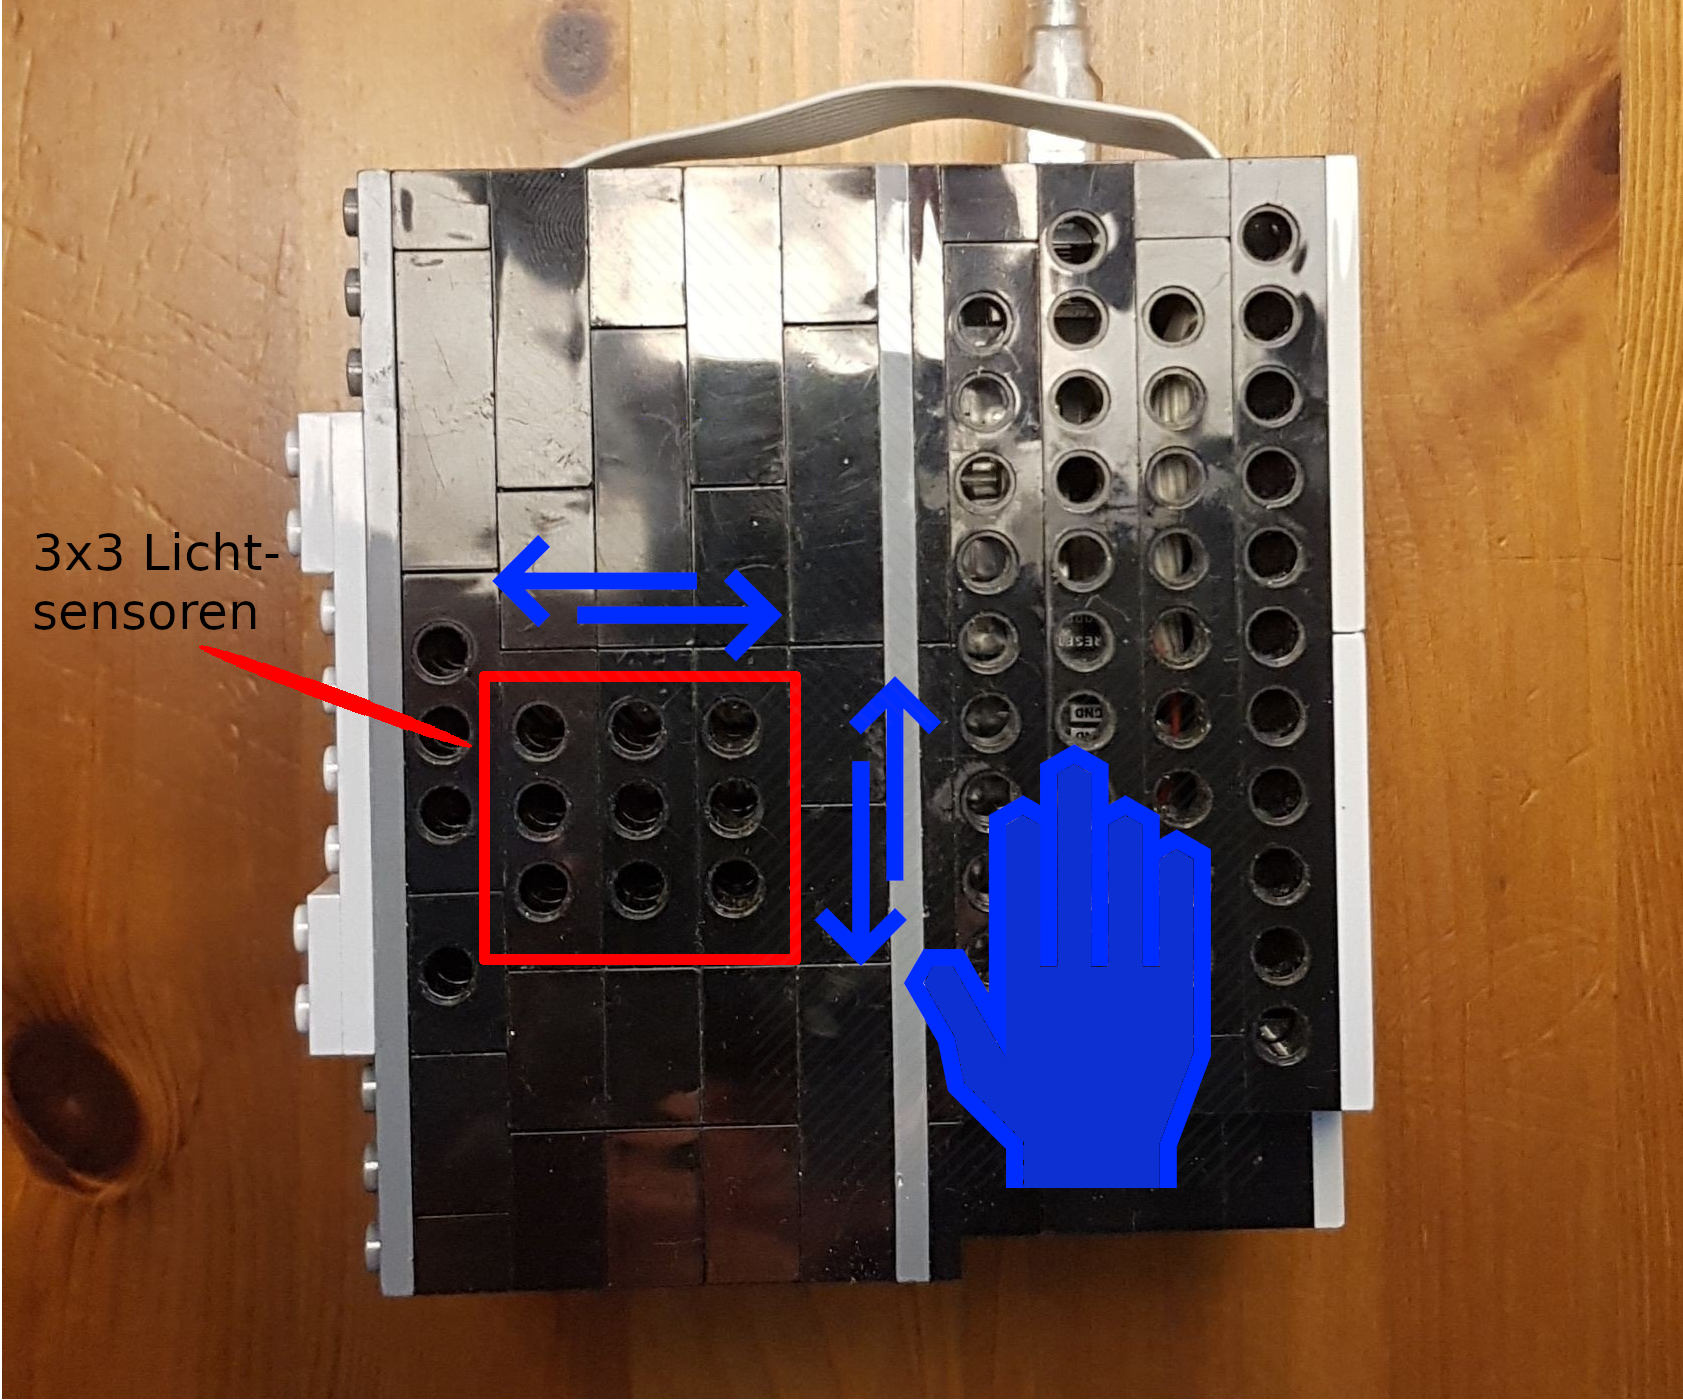
\includegraphics[width=0.77\linewidth]{aufgabe.png}
    \caption{Arduino Uno (Atmega328p) in einem Lego-Case. Illustriert 3x3 Lichtsensoren und Handgesten.}
  \end{figure}
\end{frame}

\section{Entscheidungsbäume}
\begin{frame}{Entscheidungsbäume}
\begin{figure}
    \centering
    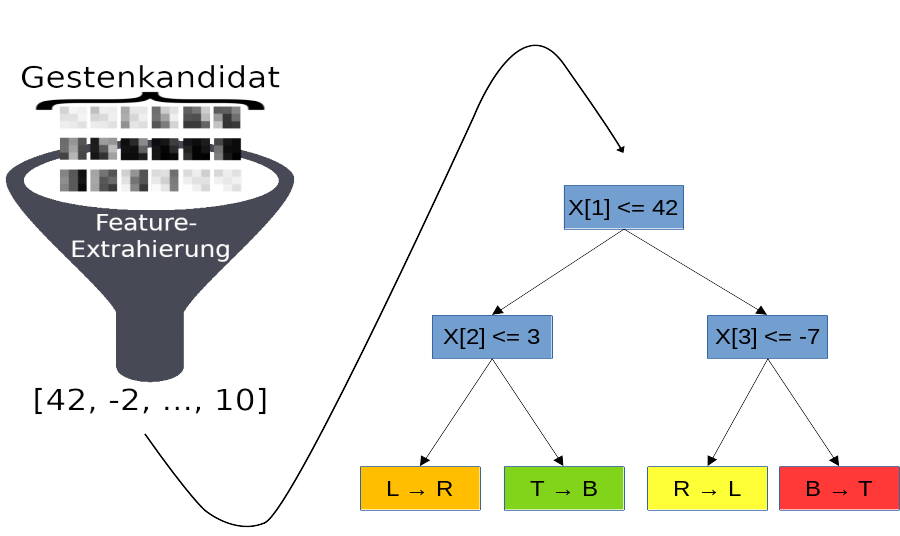
\includegraphics[width=\linewidth]{process_draw.png}
    \caption{Gestenklassifizierung eines Kandidaten mit einem Entscheidungsbaum.}
\end{figure}
\end{frame}

\section{Momentaner Stand}
\begin{frame}{Momentaner Stand}
\begin{itemize}
    \item Schwerpunktverteilung über 6 Zeitfenster
    \item Entscheidungsbaum/wald trainiert mit Scikit-Learn
    \item Trainingsset: 15\% von dataEva9Pixel, dataEva16Pixel und trainingKubik
    \item Testset: testKlisch
\end{itemize}
\end{frame}

\begin{frame}{Momentaner Stand - Schwerpunktverteilung}
\begin{figure}
    \begin{minipage}[c]{0.4\linewidth}
        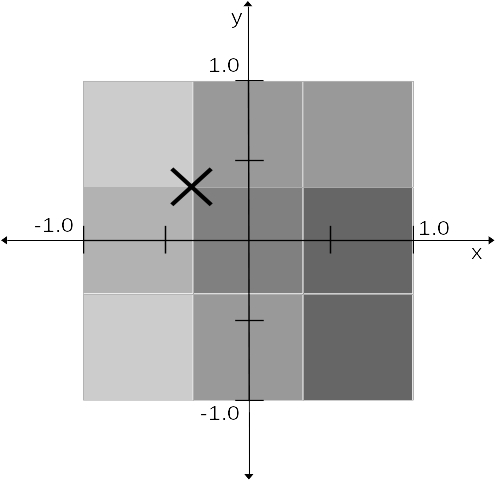
\includegraphics[width=\linewidth]{schwerpunkt_ansatz.jpg}
        \caption{Schwerpunkt eines Bildes in X und Y Richtung.}
    \end{minipage}
    \hfill
    \begin{minipage}[c]{0.4\linewidth}
        $\begin{pmatrix}
            p_{00} & p_{01} & p_{02}\\
            p_{10} & p_{11} & p_{12}\\
            p_{20} & p_{21} & p_{22}
        \end{pmatrix}$
        \\\\\\
        $P = \sum_{i,j} p_{i,j}$
        \\\\
        $X_s = \frac{\sum_{i}^{3} p_{i,0} - \sum_{i}^{3} p_{i,2}}{P}$
        \\\\
        $Y_s = \frac{\sum_{i}^{3} p_{0,i} - \sum_{i}^{3} p_{2,i}}{P}$
    \end{minipage}
\end{figure}
\begin{itemize}
    \item Komprimieren auf 6 Schwerpunkte über Durchschnitt
\end{itemize}
\end{frame}

\begin{frame}{Momentaner Stand - Schwerpunkte mit Gleitkommazahlen}
\begin{figure}
    \begin{minipage}[c]{0.4\linewidth}
        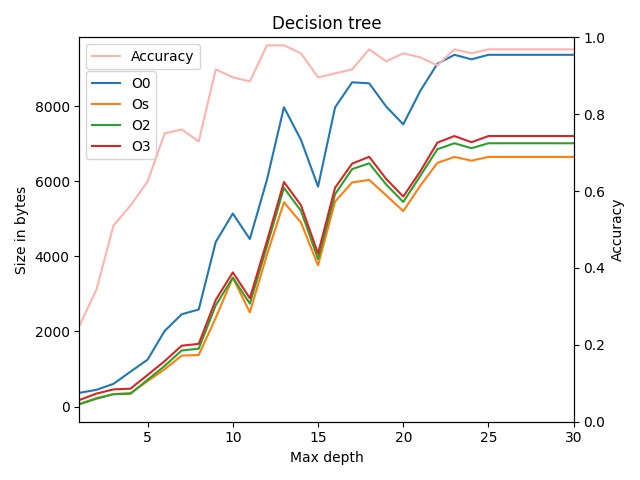
\includegraphics[width=\linewidth]{klisch_float_tree.png}
        \caption{Entscheidungsbaum Size/Accuracy über Max-Tiefe.}
    \end{minipage}
    \hfill
    \begin{minipage}[c]{0.4\linewidth}
        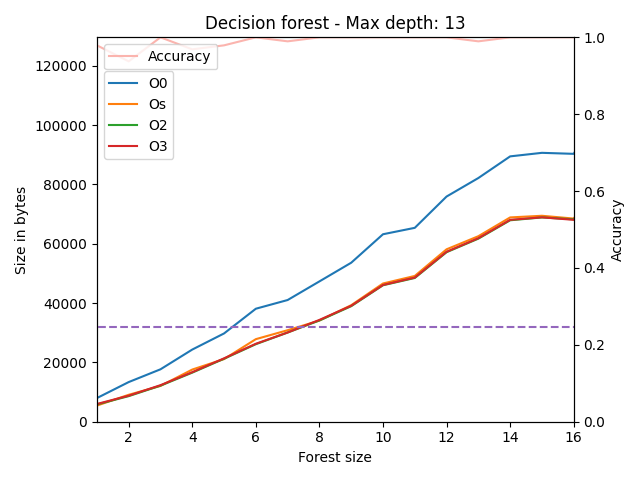
\includegraphics[width=\linewidth]{klisch_float_forest_13.png}
        \caption{Entscheidungswald Size/Accuracy über \#Bäume.}
    \end{minipage}%
\end{figure}
\begin{itemize}
    \item Baum Ausführungszeit: $\leq \hspace{0.1cm}$\#Tiefe$\hspace{0.1cm}\cdot \hspace{0.05cm} 4.1875 \mu s$
    \item Wald Overhead: $\leq 4\mu s$
    \item Feature extraction: $\leq 2(290.25\mu s + \hspace{0.05cm} $\#Bilder $ \cdot \hspace{0.1cm} 13.6875 \mu s)$
    \item Beste Konfiguration: 3 Bäume á 13 Max-Tiefe (100\% Accuracy)
    \begin{itemize}
        \item Größe in Bytes: 14576
        \item Ausführungszeit: $\leq 167.3125 \mu s$
    \end{itemize}
\end{itemize}
\end{frame}

\begin{frame}{Momentaner Stand - Schwerpunkte mit Integer}
\begin{figure}
    \begin{minipage}[c]{0.4\linewidth}
        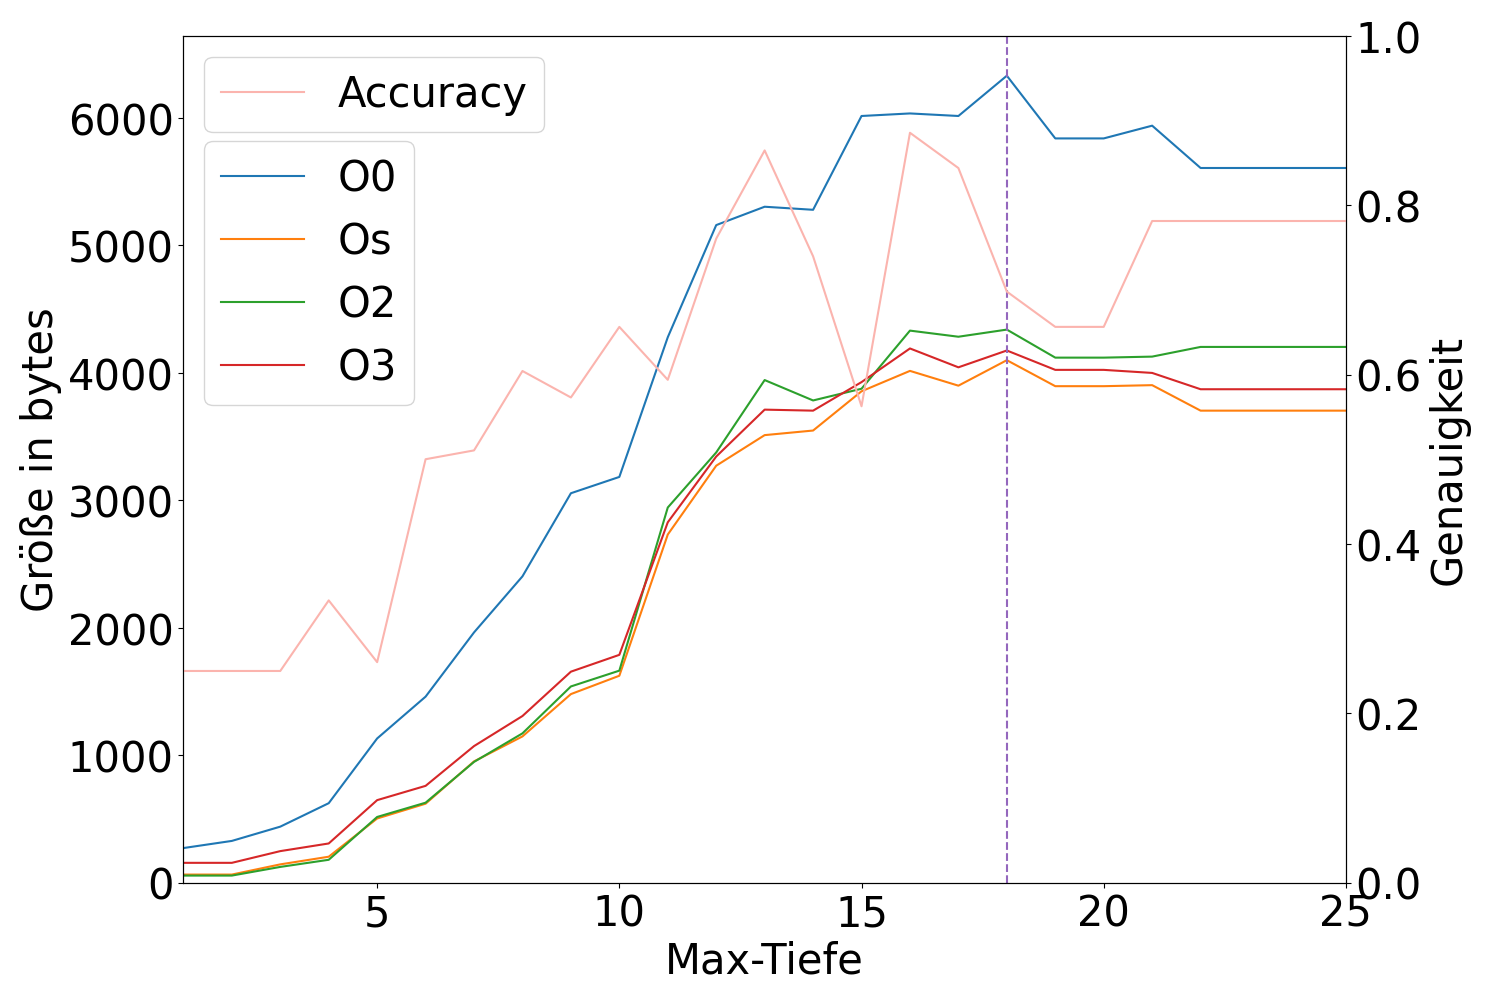
\includegraphics[width=\linewidth]{klisch_int_tree.png}
        \caption{Entscheidungsbaum Size/Accuracy über Max-Tiefe.}
    \end{minipage}
    \hfill
    \begin{minipage}[c]{0.4\linewidth}
        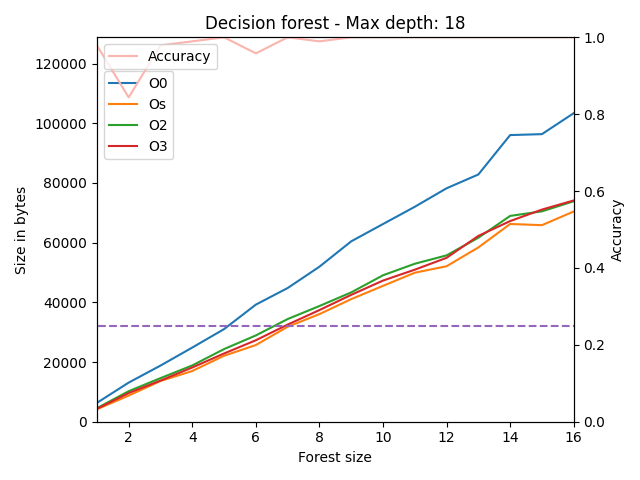
\includegraphics[width=\linewidth]{klisch_int_forest_18.png}
        \caption{Entscheidungswald Size/Accuracy über \#Bäume.}
    \end{minipage}%
\end{figure}
\begin{itemize}
    \item Baum Ausführungszeit: $\leq \hspace{0.1cm}$\#Tiefe$\hspace{0.1cm}\cdot \hspace{0.05cm} 0.9375 \mu s$
    \item Wald Overhead: $\leq 4\mu s$
    \item Feature extraction: $\leq 2(318\mu s + \hspace{0.05cm} $\#Bilder $ \cdot \hspace{0.1cm} 1.125 \mu s)$
    \item Beste Konfiguration: 5 Bäume á 18 Max-Tiefe (100\% Accuracy)
    \begin{itemize}
        \item Größe in Bytes: 24608
        \item Ausführungszeit: $\leq 88.375 \mu s$
    \end{itemize}
\end{itemize}
\end{frame}

\section{ToDo}
\begin{frame}{ToDo}
\begin{itemize}
    \item Weitere Entscheidungsbaumansätze evaluieren
    \item Nullgesten betrachten
    \item Robuster gegenüber Rotation (+- 30°)
\end{itemize}
\end{frame}

\section{Zeitplan}
\begin{frame}{Zeitplan}
\begin{figure}
    \centering
    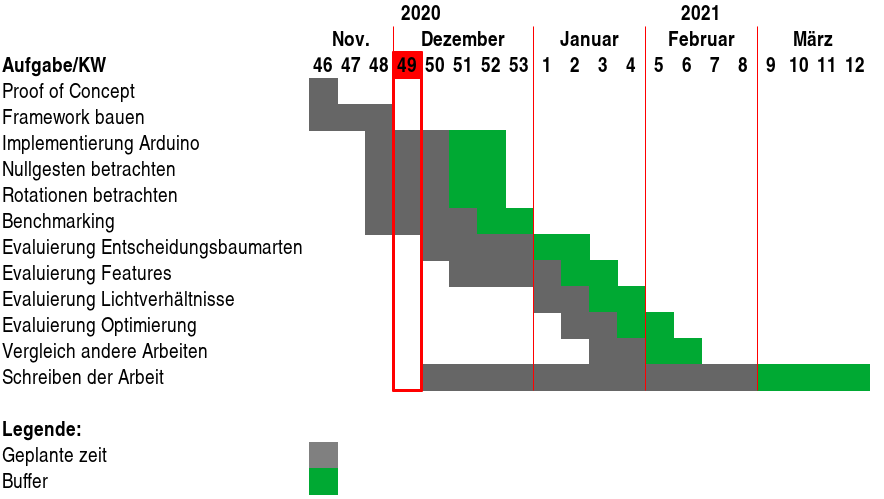
\includegraphics[width=\linewidth]{gantt_chart.png}
    \caption{Gantt Chart welches meinen Zeitplan für diese Arbeit aufzeigt.}
\end{figure}
\end{frame}
\begin{frame}[standout]
  Fragen?
\end{frame}

\end{document}
